\chapter{Pygame Invaders: Ready, set, fire!}
\label{chap:pygame-invaders-fire}
\section{Εισαγωγή}
Στο προηγούμενο κεφάλαιο ξεκινήσαμε να γράφουμε το\ldots{} όνειρο κάθε bedroom programmer των 80s: ένα γρήγορο διαστημικό space shooter.  Ειδικά η λέξη ``γρήγορο'' τις περισσότερες φορές εκείνη την εποχή σήμαινε ότι θα χρησιμοποιούσαμε assembly για την εκάστοτε πλατφόρμα μας ή ότι ήμασταν από τους τυχερούς που διέθετε μηχάνημα με hardware sprites όπως η extended BASIC του ΤΙ-99 ή ο Commodore 64.

Για τους υπόλοιπους που έγραφαν σε BASIC και περιορίζονταν σε κίνηση χαρακτήρων στην οθόνη, το Space Invaders ξεκίναγε φιλόδοξα, αλλά γρήγορα κατέληγε σε\ldots{} Space Invader αφού ζήτημα είναι να κατάφερνε να κινήσει παραπάνω από ένα εξωγήινο κάθε φορά και ταυτόχρονα να χρειάζεται να απεικονίζει και να υπολογίζει τόσο τις δικές μας κινήσεις όσο και τις βολές -- φιλικές και εχθρικές. Και δεν έχουμε ακόμα φτάσει στα ηχητικά εφέ και την ανίχνευση συγκρούσεων.

Ευτυχώς για μας, όχι μόνο τα μηχανήματα μας είναι τόσο πολύ ταχύτερα αλλά διαθέτουμε και μια γλώσσα προγραμματισμού που μπορεί να υλοποιήσει εύκολα και καθαρά ότι σκεφτούμε.

Μέχρι τώρα έχουμε δει:
\begin{itemize}
\item[-] Τις βασικές κλάσεις για το διαστημόπλοιο μας και τους εξωγήινους
\item[-] Κατεύθυνση του διαστημοπλοίου με τα βελάκια
\item[-] Μια εντελώς βασική κλάση για το φόντο
\item[-] Ήχο και μουσική στη βασική τους μορφή
\end{itemize}
%
Έχοντας φορτίσει τις προγραμματιστικές μας μπαταρίες (και όχι, στα 80s δεν συνηθίζαμε τις πίτσες και κόλες για αυτό το σκοπό) αισθανόμαστε έτοιμοι να αντιμετωπίσουμε τις επόμενες προκλήσεις του Pygame Invaders.

\begin{figure}
\centering
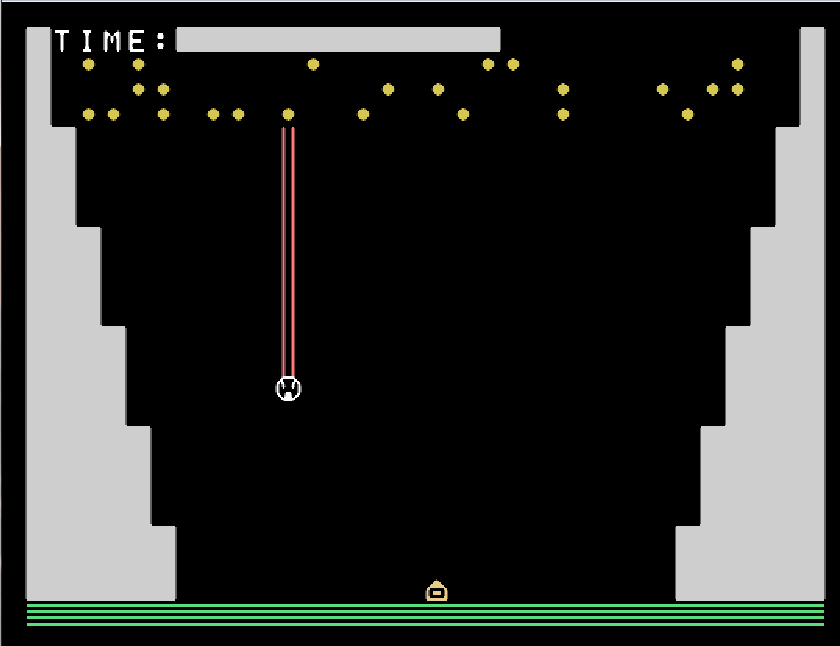
\includegraphics[width=0.8\textwidth]{images/chapter8/invaders}
\caption[Invaders]{Ο πρόγονος του προγράμματος που φτιάχνουμε εδώ θα μπορούσε να είναι το invaders που έγραψα το 1986 στον ΤΙ-99. Invaders βέβαια μόνο κατά όνομα, μιας και μετά βίας έβγαζε\ldots{} ένα εξωγήινο κάθε φορά. Λογικό όμως: Laser, διαστημόπλοιο, εξωγήινος, κίνηση, ήχος και score σε\ldots{} 3Mhz είναι απλά θαύμα. Και βέβαια είναι γραμμένο σε BASIC, με κίνηση χαρακτήρων, χωρίς καν sprites\ldots{} Give me a break!}
\label{8-1}
\end{figure}
%
\section{Κυλιόμενο Φόντο}
%
Μια απίστευτη πρόκληση για τα 80s, το κυλιόμενο φόντο στο δικό μας παιχνίδι δεν είναι κάτι τόσο δύσκολο πλέον. Πως όμως θα δημιουργήσουμε μια κυλιόμενη εικόνα από μια στατική, και μάλιστα όταν το μέγεθος της στατικής είναι όσο το παράθυρο μας;

Φανταστείτε πολύ απλά, ότι παίρνετε την εικόνα του φόντου και σε κάθε καρέ τη μετατοπίζετε προς τα κάτω – με μια συγκεκριμένη ταχύτητα φυσικά. Ας ξεκινήσουμε λοιπόν με αυτή την απλή εκδοχή να γράψουμε την {\tt Scroll}, την οποία την είχαμε αφήσει με ένα μοναχικό {\tt pass}:

\begin{minted}[bgcolor=bg, frame=lines, framesep=10pt]{python}
  def Scroll(self, speed_y, time):
    distance_y = speed_y * time
    self.coord[1] += distance_y
\end{minted}

Στο κύριο πρόγραμμα μας, θα προσθέσουμε φυσικά και την αντίστοιχη γραμμή πάνω από το {\tt StarField.Show(screen)}:

\begin{minted}[bgcolor=bg, frame=lines, framesep=10pt]{python}
    StarField.Scroll(backspeed, time)
\end{minted}

Αρκεί να ορίσουμε κάπου και την επιθυμητή ταχύτητα, {\tt backspeed} σε μια γραμμή που θα βάλουμε οπουδήποτε έξω από το βασικό βρόχο {\tt while} του παιχνιδιού μας:

\begin{minted}[bgcolor=bg, frame=lines, framesep=10pt]{python}
  # Set the background scrolling speed

  backspeed = 100
\end{minted}

Αυτό είναι! Ας το τρέξουμε τώρα, και καλωσορίσατε στο\ldots{}
%
\subsection{Python Debugging!}
%
Όπως έχουμε ήδη πει, όχι μόνο θα αλλάξουμε τον κώδικα μας αρκετές φορές μέχρι να πετύχουμε το αποτέλεσμα που θέλουμε, αλλά θα πρέπει να διορθώσουμε και τα προβλήματα του, ακόμα περισσότερες! Δεν υπάρχει κώδικας που είναι αλάνθαστος από την πρώτη φορά.

Αν δοκιμάσατε να τρέξετε το προηγούμενο, θα είδατε:
%
\begin{verbatim}
Traceback (most recent call last):
  File "pygame-invaders.py", line 126, in <module>
    StarField.Scroll(backspeed, time)
  File "pygame-invaders.py", line 58, in Scroll
    self.coord[1] += distance_y
TypeError: 'tuple' object does not support item assignment
\end{verbatim}
%
Με απλά λόγια: προσπαθήσαμε να αλλάξουμε τη μεταβλητή {\tt self.coord}, μόνο που αυτή την είχαμε ορίσει στο βασικό μας πρόγραμμα ως tuple. Θυμηθείτε, τα tuples σε αντίθεση με τις λίστες δεν αλλάζουν (\emph{immutable objects} τα ονομάζει η python). Ας το αλλάξουμε αυτό λοιπόν. Βρείτε τη γραμμή:

\begin{minted}[bgcolor=bg,  frame=lines, framesep=10pt]{python}
  StarField = SpaceBackground((0,0), "stars.jpg")
\end{minted}

και αλλάξτε τη σε:

\begin{minted}[bgcolor=bg,  frame=lines, framesep=10pt]{python}
  StarField = SpaceBackground([0,0], "stars.jpg")
\end{minted}

Αλλάζοντας τις παρενθέσεις σε αγκύλες, μετατρέψαμε το tuple σε λίστα. Μπορούμε τώρα να τρέξουμε ξανά το πρόγραμμα.

\begin{SCfigure}
\centering
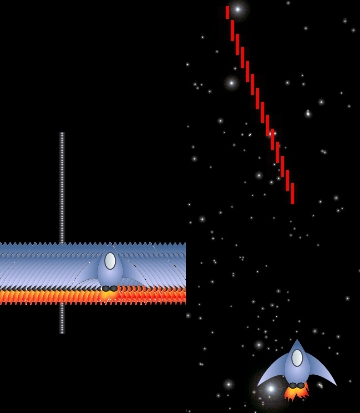
\includegraphics[width=0.5\textwidth]{images/chapter8/mess}
\caption[Χαλασμένο Laser!]{Μην αφήσετε κανένα προγραμματιστή να σας πείσει ότι ο κώδικας του είναι τέλειος ή --- ακόμα χειρότερα --- ότι δουλεύει με την πρώτη. Αριστερά, μείναμε από\ldots{} φόντο καθώς τα αστέρια κύλησαν κάτω από την οθόνη πριν γράψουμε τη ρουτίνα που κάνει την εικόνα\ldots{} ρολό. Αναμέναμε ότι θα δούμε κάτι περίεργο βέβαια. Δεξιά, το διαστημόπλοιο μας ρίχνει συνεχόμενες, κολλημένες μεταξύ τους βολές. Η αρχική μας σχεδίαση είχε κάποια\ldots{} εχμ\ldots{} μικροπροβλήματα.}
\label{8-3}
\end{SCfigure}
%
\section{Scrolling Background, Απόπειρα II}

Μη φωνάξετε ``χάλια'' μόλις δείτε το αποτέλεσμα\ldots{} Περιμένατε μήπως δια μαγείας το φόντο να επαναλαμβάνεται; Απλά στην τωρινή εκδοχή το μόνο που γίνεται είναι να σκρολλάρει και τελικά να εξαφανίζεται στο κάτω μέρος του παραθύρου. Ακόμα πιο ενοχλητική είναι η γραμμή που μένει από εκείνο το μοναχικό αστεράκι -- για να μην πούμε ότι η κίνηση του διαστημοπλοίου καταστρέφεται μόλις εξαφανιστεί το φόντο: είναι λογικό, καθώς το φόντο ουσιαστικά ``σβήνει'' το προηγούμενο καρέ πριν εμφανιστεί το επόμενο. Όταν αυτό δεν γίνεται πλέον, το ένα καρέ πέφτει επάνω στο άλλο, με το σουρεαλιστικό αποτέλεσμα που βλέπετε στην εικόνα \ref{8-3}. Ακόμα και ο James T. Kirk δεν είχε φανταστεί τέτοια κατάληξη για το USS Enterprise!

Εύκολο να το φτιάξουμε όμως: τι θέλουμε στην πραγματικότητα;  Να κολλήσουμε δύο εικόνες φόντου, ώστε να φτιάξουμε ένα ``ρολό''.
%
\begin{itemize}
\item[-] Η πρώτη εικόνα απεικονίζεται στο [0,0] και η δεύτερη ακριβώς πάνω από αυτή -- η δεύτερη δηλ. θα τελειώνει στο [0,0] και αρχικά θα είναι αόρατη!
\item[-] Η κίνηση γίνεται προς τα κάτω και για τις δύο, ταυτόχρονα.
\item[-] Όταν η πρώτη εικόνα φτάσει στο κάτω άκρο του παραθύρου, η δεύτερη πλέον εικόνα είναι σε πλήρη εμφάνιση στο παράθυρο μας.
\item[-] Η διαδικασία επαναλαμβάνεται από την αρχή και κανείς δεν καταλαβαίνει ότι είναι το ίδιο φόντο!
\end{itemize}
%
%
\section{Scrolling Background, Απόπειρα III}
%
Ας ξαναδούμε λοιπόν την κλάση για το background, σύμφωνα με τα παραπάνω, με σχόλια ανάμεσα στον κώδικα:

\begin{minted}[bgcolor=bg, frame=lines, framesep=10pt]{python}
class SpaceBackground:
  def __init__(self, coord, coord2, imagefile):
\end{minted}

Προσθέσαμε μια λίστα {\tt coord2} που θα περιέχει τις συντεταγμένες της δεύτερης εικόνας. Αρχικά θα έχει τιμή {\tt [0, -screenheight]}, όπως θα ορίσουμε κατά τη δημιουργία του αντικειμένου και θα είναι αόρατη.

\begin{minted}[bgcolor=bg, linenos, frame=lines, framesep=10pt]{python}
    self.shape = pygame.image.load(imagefile)
    self.coord = coord
    self.coord2 = coord2
    self.y_original = coord[1]
    self.y2_original = coord2[1]
\end{minted}

Αποθηκεύουμε τις αρχικές συντεταγμένες γραμμής και για τις δύο εικόνες. Η κίνηση των εικόνων αλλάζει ακριβώς αυτές τις τιμές και μόλις ολοκληρωθεί ένα πλήρες scroll πρέπει να μπορούμε να επανέλθουμε σε αυτές. 

\begin{minted}[bgcolor=bg, frame=lines, framesep=10pt]{python}
  def Show(self, surface):
    surface.blit(self.shape, self.coord)
    surface.blit(self.shape, self.coord2)
\end{minted}

Προσθέσαμε ακόμα μια γραμμή που κάνει blit και την δεύτερη εικόνα. Τίποτα το ιδιαίτερο.

\begin{minted}[bgcolor=bg, linenos, frame=lines, framesep=10pt]{python}
  def Scroll(self, speed_y, time):
    distance_y = speed_y * time
    self.coord[1] += distance_y
    self.coord2[1] += distance_y
\end{minted}

Παρόμοια, εδώ προσθέσαμε μια γραμμή για να κινείται και η δεύτερη εικόνα. Αλλά όλο το παιχνίδι παίζεται εδώ: 

\begin{minted}[bgcolor=bg, frame=lines, framesep=10pt]{python}
    if self.coord2[1] >= 0:
      self.coord[1] = self.y_original
      self.coord2[1] = self.y2_original
\end{minted}

Μόλις η δεύτερη εικόνα εμφανιστεί πλήρως στην οθόνη (φτάσει δηλ. στο [0,0] ή λόγω\ldots{} κεκτημένης ταχύτητας το ξεπεράσει!), επανερχόμαστε στις αρχικές συντεταγμένες και για τις δύο εικόνες. Τώρα αν αυτό δεν είναι καμπύλωση του χωροχρόνου, δεν ξέρω τι είναι! Τρέμε Αϊνστάιν!

Στο κύριο πρόγραμμα μας, η δημιουργία του αντικειμένου για το φόντο γίνεται πλέον με τη γραμμή:

\begin{minted}[bgcolor=bg, frame=lines, framesep=10pt]{python}
  StarField = SpaceBackground([0,0],[0, -screenheight], "stars.jpg")
\end{minted}

\begin{SCfigure}
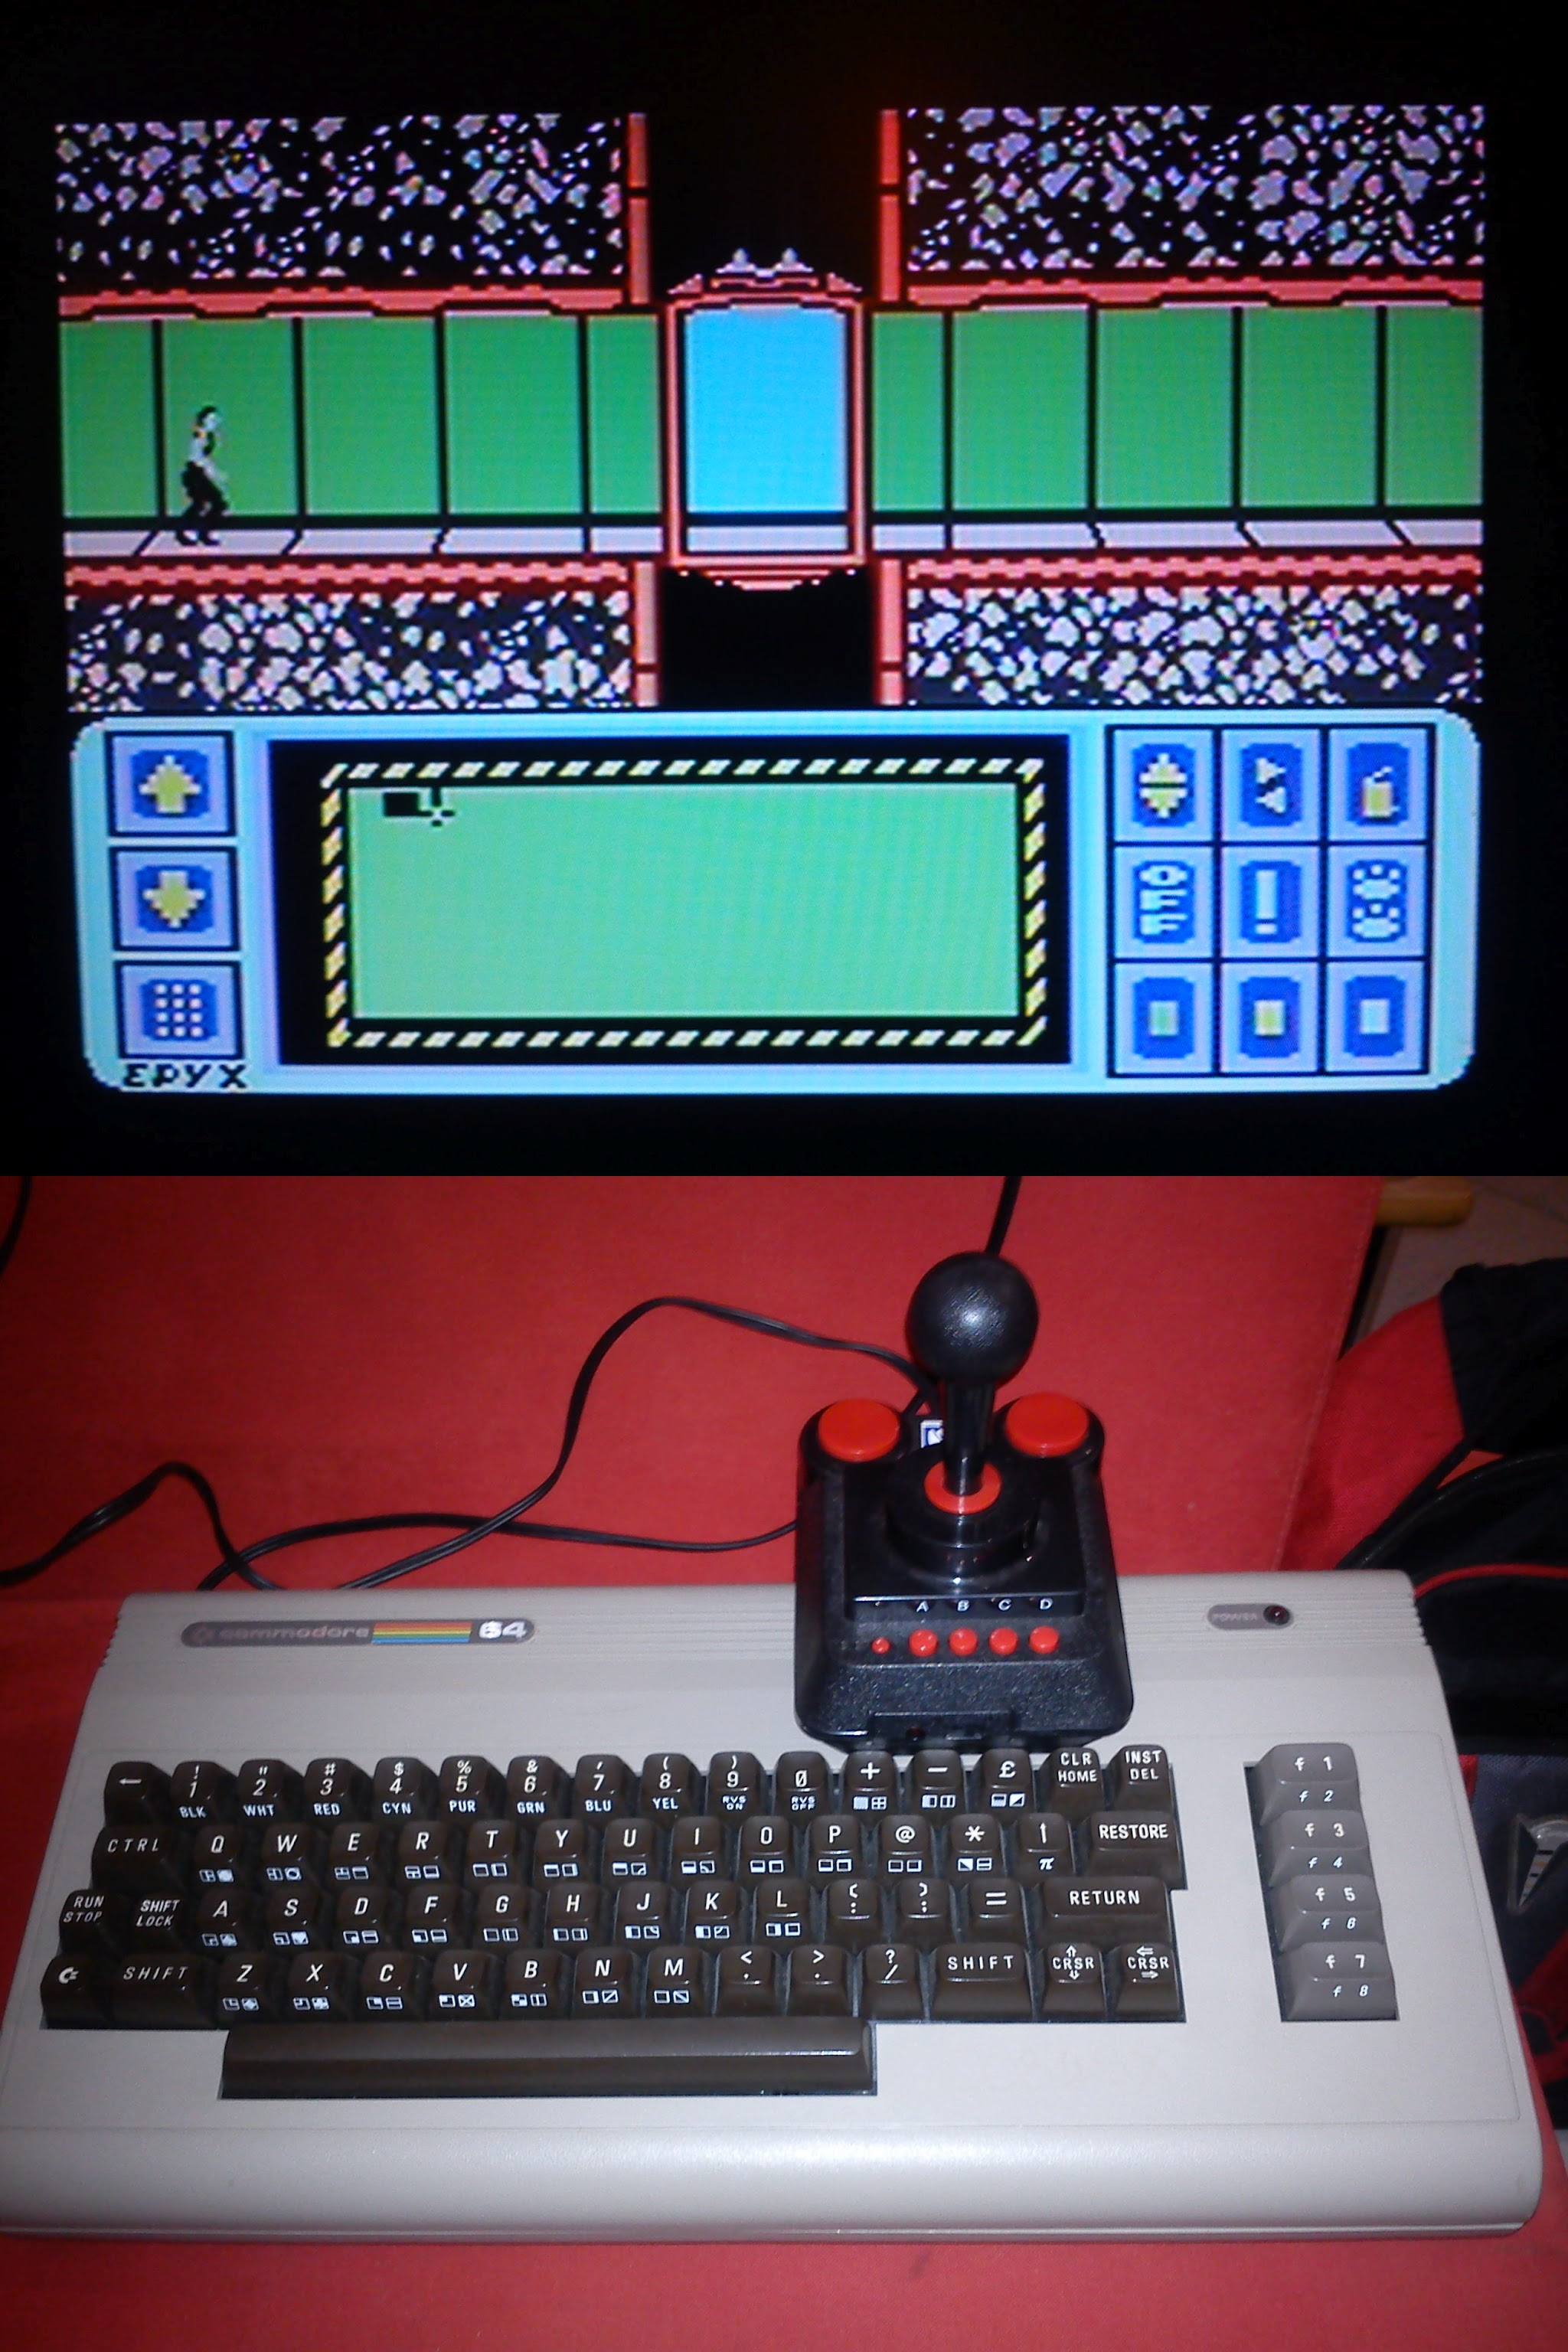
\includegraphics[width=0.4\textwidth]{images/chapter8/c64dtv}
\caption[Commodore 64 Direct to TV]{Το μηχάνημα είναι ο γνωστός Commodore 64, ο υπολογιστής με τις περισσότερες πωλήσεις όλων των εποχών! Αν νομίζετε όμως ότι το joystick που φαίνεται προορίζεται να συνδεθεί πάνω του, χάσατε! Δεν είναι ένα απλό joystick, είναι το C64DTV: περιέχει μέσα του ένα  ολόκληρο C64 (ΟΚ, χωρίς το πληκτρολόγιο) και κάμποσα παιχνίδια (από αυτά που φορτώναμε τότε με τις ώρες) σε μια ROM. Λειτουργεί με μπαταρίες και συνδέεται απευθείας στην τηλεόραση σας. Ναι, όλος ο C64 με σημερινή τεχνολογία χωράει σε 2 τσιπάκια στο κάτω μέρος ενός joystick! Εκπληκτικό – αλλά εμείς βέβαια προτιμάμε τη μαγεία του αρχικού. Στην πάνω εικόνα το διάσημο παιχνίδι Mission Impossible του C64 από το C64DTV.}
\label{8-2}
\end{SCfigure}
%
\section{Fire the Lasers!}
%
Έχοντας επιτέλους τελειώσει με το φόντο, ήρθε η ώρα να διαλύσουμε τους εξωγήινους με το Laser μας. Το γεγονός ότι το παιχνίδι μας δεν δείχνει ακόμα εξωγήινους, είναι μια μικρή ενοχλητική λεπτομέρεια. Τι θέλετε δηλαδή, να φτιάξουμε πρώτα τους εξωγήινους και να μην έχουμε όπλα; Θα φεύγατε για πόλεμο χωρίς δοκιμαστικές βολές και εκπαίδευση;

Τώρα λοιπόν που λογικευτήκατε, ας δούμε τι θα πρέπει να περιέχει μια κλάση για το Laser:
%
\begin{itemize}
\item[-] Κλασικά, ένα constructor. Θα ορίζει και μερικές βασικές παραμέτρους: αρχικές συντεταγμένες, χρώμα, μήκος της γραμμής, ταχύτητα.
\item[-] {\tt Show}: Για να εμφανιστεί η βολή στην επιφάνεια της επιλογής μας
\item[-] Μια συνάρτηση {\tt Move} για την κίνηση της βολής.
\end{itemize}
%
Σε μια πρώτη σκέψη, ίσως τα παραπάνω σας φαίνονται αρκετά. Να σας ρωτήσω όμως: Πότε εξαφανίζεται μια βολή; Σε δύο περιπτώσεις:
%
\begin{enumerate}
\item Όταν χτυπήσει τον επάρατο εχθρό μας
\item Όταν βγει έξω από την οθόνη μας
\end{enumerate}
%
Δεν έχουμε ακόμα εχθρούς, αλλά χρειάζεται να κάνουμε κάτι για το (2).

Χρειαζόμαστε ακόμα μια συνάρτηση που να δείχνει αν η βολή έχει φύγει πάνω από την οθόνη.  Προφανώς, αρκεί να επιστρέφει {\tt True} ή {\tt False}.
Ας κάνουμε λοιπόν μια πρώτη απόπειρα.
%
\section{Laser Class}
%
Σχετικά εύκολα μπορούμε να υλοποιήσουμε την κλάση που περιγράψαμε. Ας δούμε τον κώδικα μας με τα σχετικά σχόλια:

\begin{minted}[bgcolor=bg, linenos, frame=lines, framesep=10pt]{python}
class Laser:
  def __init__(self, coord, color, size, speed):
    self.x1 = coord[0]
    self.y1 = coord[1]
    self.size = size
    self.color = color
    self.speed = speed
\end{minted}

O constructor δίνει τις αρχικές συντεταγμένες ({\tt coord}) οι οποίες μπορεί να είναι tuple ή λίστα, το χρώμα (σε μορφή λίστας RGB), το μέγεθος ({\tt size}) και την ταχύτητα κίνησης ({\tt speed}). Οι συντεταγμένες ανατίθενται απευθείας σε χωριστές μεταβλητές {\tt x1} και {\tt y1} για να τις επεξεργαζόμαστε εύκολα σε όλες τις υπόλοιπες συναρτήσεις. 

\begin{minted}[bgcolor=bg, frame=lines, framesep=10pt]{python}
  def Show(self, surface):
    pygame.draw.line(surface, self.color, (self.x1,self.y1),(self.x1,self.y1-self.size),3)
\end{minted}

Η συνάρτηση {\tt Show} είναι απλή: χρησιμοποιούμε την {\tt draw} του pygame για να φτιάξουμε μια γραμμή στο κατάλληλο μέγεθος και χρώμα. Οι συντεταγμένες δίνονται με τη μορφή δύο tuples (αρχής και τέλους γραμμής) και καθώς βλέπετε το μόνο που κάνουμε είναι να αλλάζουμε το {\tt y1} για το κατάλληλο μήκος γραμμής. Το\ldots{} μυστηριώδες 3 στο τέλος είναι το πλάτος της γραμμής, τρία pixels. Αν θέλαμε να είμαστε σωστότεροι θα το ορίζαμε στον constructor (της νύχτας τον κώδικα τον βλέπει η μέρα και γελά).

\begin{minted}[bgcolor=bg, frame=lines, framesep=10pt]{python}
  def Move(self, time):
    distance = self.speed * time
    self.y1 += distance
\end{minted}

Δεν νομίζουμε ότι η {\tt Move} χρειάζεται πρακτικά κάποια εξήγηση!

\begin{minted}[bgcolor=bg, linenos, frame=lines, framesep=10pt]{python}
  def GoneAbove(self,y):
    if self.y1<=y:
      return True
    else:
      return False
\end{minted}

Η συνάρτηση {\tt GoneAbove} θα μας λέει αν η βολή έχει πάει πάνω από κάποιο όριο της οθόνης -- αν έχει βγει από την οθόνη θα πρέπει να την σβήσουμε.

Πιστεύετε ότι έχουμε κάνει καλή δουλειά και το Laser μας θα λειτουργήσει με την πρώτη. Πόσο γελασμένοι είστε. Ευτυχώς που δεν σας έβαλα ακόμα εξωγήινους, θα σας είχαν φάει λάχανο! Αλλά ας μείνουμε λίγο ακόμα στην άγνοια μας, και πάμε να δούμε πως θα ενσωματώσουμε αυτό το --- θεός να το κάνει --- όπλο στο κύριο πρόγραμμα μας.
%
\section{Συνάρτηση Fire στο Craft class}
%
Η βολή είναι προφανώς μια δυνατότητα στο {\tt Craft} class.  Αν το σκεφτείτε, δεν χρειάζεται να φτιάξουμε διαφορετικό Laser class για τους εξωγήινους, άρα μας βολεύει να φτιάξουμε την μέθοδο {\tt Fire} στο superclass.  Θα πρέπει όμως να προσθέσουμε κάποια πράγματα στον constructor του {\tt Craft}:

\begin{minted}[bgcolor=bg, linenos, frame=lines, framesep=10pt]{python}
class Craft(object):
  def __init__ (self, imagefile, coord):
    self.shape = pygame.image.load(imagefile)
    self.ship_width = self.shape.get_width()
    self.ship_height = self.shape.get_height()
    self.rect = pygame.Rect(coord,(self.ship_width, self.ship_height))
    self.ship_midwidth = self.ship_width / 2
    self.firecolor=(255,0,0)
    self.firespeed = -800
    self.shotlength = 20
\end{minted}

Προσθέσαμε τις τέσσερις τελευταίες γραμμές. To {\tt midwidth} είναι ακριβώς αυτό που λέει: το μισό πλάτος του διαστημοπλοίου. Καθώς φαντάζεστε, το Laser θα πρέπει να φεύγει από τη μύτη του διαστημοπλοίου μας που βρίσκεται στη μέση! Το χρώμα της βολής θα είναι κόκκινο (255,0,0) και η ταχύτητα -800. Μη σας παραξενεύει η αρνητική τιμή: το Laser κινείται από κάτω προς τα πάνω! Και πάμε να δούμε τη συνάρτηση {\tt Fire}:

\begin{minted}[bgcolor=bg, frame=lines, framesep=10pt]{python}
  def Fire(self):
    shot = Laser((self.rect[0]+self.ship_midwidth, self.rect[1]), 
                  self.firecolor,self.shotlength,self.firespeed)
    return shot
\end{minted}

Με το {\tt midwidth} εξασφαλίζουμε ότι η βολή θα βγει από τη μέση του διαστημοπλοίου, τη μύτη του! Η συνάρτηση επιστρέφει ένα αντικείμενο τύπου\ldots{} Laser. Ο λόγος θα γίνει προφανής σε λίγο.
%
\subsection{Πρώτη Απόπειρα}
%
Δείχνοντας υπερβολική εμπιστοσύνη στον εαυτό μας, είμαστε έτοιμοι για την πρώτη δοκιμή. Μένουν μόνο κάποιες γραμμές στο κύριο πρόγραμμα.

\begin{minted}[bgcolor=bg, frame=lines, framesep=10pt]{python}
        if key[K_SPACE]:
          firelist.append(SpaceShip.Fire())
\end{minted}

Φαντάζεστε βέβαια που βρίσκεται αυτή η γραμμή, αλλά τι είναι το {\tt firelist}; Μα το διαστημόπλοιο μας μπορεί να ρίξει πολλές βολές. Δεν χρειάζεται να εξαφανιστεί η προηγούμενη για να ρίξουμε νέα! Πως λοιπόν θα κρατήσουμε λογαριασμό για τις βολές που πρέπει να σχεδιάσουμε στην επιφάνεια μας; Κάθε φορά που ρίχνουμε βολή το αντικείμενο που επιστρέφει η {\tt Fire} αποθηκεύεται στην λίστα {\tt firelist}. Προφανώς την έχουμε αρχικοποιήσει έξω από το βρόχο {\tt while} με την εντολή:

\begin{minted}[bgcolor=bg, frame=lines, framesep=10pt]{python}
  firelist = []
\end{minted}

Είναι έπειτα πολύ εύκολο να την κινήσουμε και να την δείξουμε, προσθέτοντας τις παρακάτω γραμμές μετά το {\tt SpaceShip.Show(screen)}:

\begin{minted}[bgcolor=bg, frame=lines, framesep=10pt]{python}
    for theshot in firelist:
      theshot.Move(time)
\end{minted}

Για κάθε βολή που έχουμε προσθέσει στη λίστα, την κινούμε.

\begin{minted}[bgcolor=bg, frame=lines, framesep=10pt]{python}
      theshot.Show(screen)
\end{minted}

Την δείχνουμε.

\begin{minted}[bgcolor=bg, frame=lines, framesep=10pt]{python}
      if theshot.GoneAbove(0):
        firelist.remove(theshot)
\end{minted}

Ερευνούμε αν έχει βγει πάνω από την οθόνη, και αν συμβαίνει αυτό την αφαιρούμε από τη λίστα.

Τρέξτε το λοιπόν και δείτε το αποτέλεσμα. Αν δεν θέλετε να ντροπιαστείτε στο Υπεργαλακτικό Συνέδριο Κβαντικής Τεχνολογίας, δείτε απλώς την εικόνα \ref{8-3}. Τι είναι αυτές οι συνεχόμενες γραμμές; Εμείς για Laser ξεκινήσαμε και μάλιστα με μήκος 20 pixels. Αλλά αν πιέζετε το {\tt SPACE} (το πλήκτρο ενεργοποίησης) συνέχεια θα έχετε μια\ldots{} συνεχόμενη γραμμή προς τα πάνω (θυμίζει λίγο το Parsec, το παιχνίδι του TI-99 που φαίνεται στην εικόνα). Μη ξεχνάτε έχουμε ρυθμίσει το πληκτρολόγιο στη μέγιστη επανάληψη. Τι μπορούμε να κάνουμε;
%
\subsection{Δεύτερη Απόπειρα}
%
Εντάξει, για πρώτη απόπειρα δεν τα πήγαμε τόσο άσχημα, το φιάσκο με το φόντο ήταν σαφώς μεγαλύτερο. Χρειάστηκε να σκεφτούμε πολλά πράγματα και μας διέφυγε μόνο ένα:
%
\begin{itemize}
\item Το διαστημόπλοιο δεν πρέπει να ρίχνει νέα βολή αν η προηγούμενη δεν έχει ``ταξιδέψει'' μια ελάχιστη απόσταση από το αρχικό σημείο.
\end{itemize}
%
Και πως θα γίνει αυτό; Μα φυσικά θα φτιάξουμε μια συνάρτηση που θα δίνει την απόσταση της βολής από ένα σημείο αναφοράς (τη γραμμή που βρίσκεται το σκάφος μας τη στιγμή που ρίχνει τη βολή). Στον constructor του {\tt Laser} θα έχουμε μια επιπλέον παράμετρο για την γραμμή αναφοράς:

\begin{minted}[bgcolor=bg, frame=lines, framesep=10pt]{python}
class Laser:
  def __init__(self, coord, color, size, speed, refline):
\end{minted}

και θα αποθηκεύσουμε προφανώς αυτή την τιμή:

\begin{minted}[bgcolor=bg, frame=lines, framesep=10pt]{python}
    self.refline = refline
\end{minted}

και η συνάρτηση μας θα είναι:

\begin{minted}[bgcolor=bg, frame=lines, framesep=10pt]{python}
  def DistanceTravelled(self):
    return self.refline - self.y1
\end{minted}

Η μέθοδος {\tt Fire} θα πρέπει να ορίζει το {\tt refline}, ως την τρέχουσα γραμμή του διαστημοπλοίου μας:

\begin{minted}[bgcolor=bg, frame=lines, framesep=10pt]{python}
  def Fire(self):
    shot = Laser((self.rect[0]+self.ship_midwidth, self.rect[1]),
                  self.firecolor,self.shotlength,self.firespeed,self.rect[1])
    return shot
\end{minted}

και τέλος η ανίχνευση πληκτρολογίου αλλάζει ως εξής:

\begin{minted}[bgcolor=bg, linenos, frame=lines, framesep=10pt]{python}
        if key[K_SPACE]:
          if firelist:
            # Only fire if last shot has travelled a minimum distance
            if firelist[-1].DistanceTravelled() >=  150:
              firelist.append(SpaceShip.Fire())
          else:
            # or if there is no shot
            firelist.append(SpaceShip.Fire())
\end{minted}

Απλά, το διαστημόπλοιο δεν ρίχνει αν η τελευταία βολή (το {\tt firelist[-1]} πολύ βολικά μας επιστρέφει το τελευταίο στοιχείο της λίστας) δεν έχει ταξιδέψει τουλάχιστον 150 pixels από τη γραμμή βολής. Αν βέβαια δεν υπάρχει καμιά βολή (περίπτωση {\tt else}), το διαστημόπλοιο ρίχνει αμέσως. Αλλάζοντας το 150 θα μπορείτε να ελέγξετε την ``πυκνότητα'' αν θέλετε των βολών (cheat mode on!)

\begin{figure}
\centering
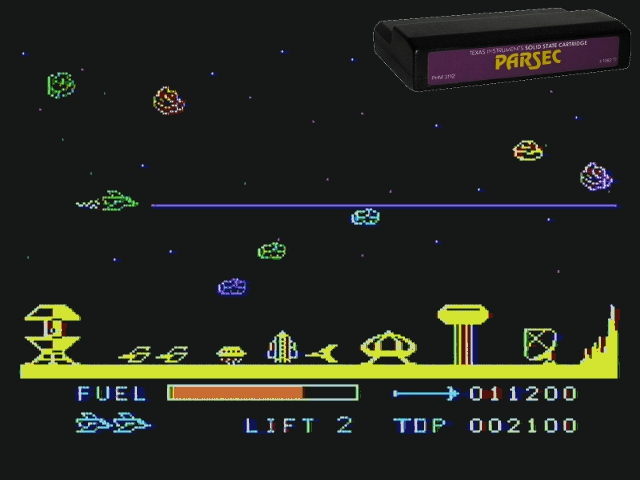
\includegraphics[width=0.8\textwidth]{images/chapter8/parsec}
\caption[Parsec]{Από τα πλέον διάσημα παιχνίδια σε cartridge του TI-99/4A, το Parsec είναι ένα διαστημικό παιχνίδι με side scrolling, σταθμούς ανεφοδιασμού, πολλαπλές πίστες και εκείνο το συνεχόμενο Laser που κάτι μας θυμίζει! Ένα ακόμα εκπληκτικό προσόν του ήταν η ομιλία -- για όποιον τυχερό είχε το speech synthesizer. Για τους πραγματικά παλιούς από σας, το Parsec ήταν το επίσημο video game του εφηβικού τηλεπαιχνιδιού ``Κόκκινοι γίγαντες, άσπροι νάνοι'' που βλέπαμε μετά μανίας στην κρατική τηλεόραση!}
\label{8-4}
\end{figure}
%
\section{Ήχος Βολής!}
%
Χάρις στην {\tt PrepareSound}, είναι εύκολο να κάνουμε το Laser μας\ldots{} θορυβώδες. Τι είπατε, στο διάστημα δεν έχει αέρα και άρα δεν ακούγεται ήχος; Γιατί μήπως τα αστέρια είναι δύο εικόνες κολλημένες σε ρολό που γυρίζουν; Σας παρακαλώ, αφήστε με στην φαντασία μου! Σε ένα βολικό σημείο πριν το βασικό βρόχο γράφουμε:

\begin{minted}[bgcolor=bg,  frame=lines, framesep=10pt]{python}
  laser = PrepareSound("shoot.wav")
\end{minted}

Μπορούμε να προσθέσουμε τον ήχο απευθείας στη συνάρτηση {\tt Fire} του {\tt Craft} class:

\begin{minted}[bgcolor=bg,  frame=lines, framesep=10pt]{python}
    laser.play()
\end{minted}

Το παιχνίδι μας επιτέλους αρχίζει να παίρνει μορφή! Έχουμε το κινούμενο φόντο, έχουμε το Laser, έχουμε κίνηση. Μένει να υποδεχτούμε μόνο τους (χαμένους από χέρι) εξωγήινους, το οποίο θα γίνει πολύ σύντομα.
